\chapter{Análisis del Diseño del Sistema}
\label{Análisis del Diseño del Sistema}

\section{Introducción}
Luego de haber adquirido una cantidad de conocimiento sobre Detección de Objetos en general y sobre el algoritmo de YOLO en particular, el presente capitulo 
investiga los problemas que tiene el área agropecuaria y la necesidad de detección y de localización de las silobolsas y mecanismos de riego por pivotes. Para esto, se realizó una entrevista con las partes interesadas o stakeholders en hacer uso de la aplicación resultante de este trabajo final, donde manifestaron su importancia. Luego se procede a analizar si las soluciones propuestas a las cuales se llegaron en la entrevista representan un caso de uso de Detección de Objetos. Por último, se especifican Componentes, Requerimientos y Comportamiento del sistema a implementar.
\begin{figure}[h!]
    \centering
    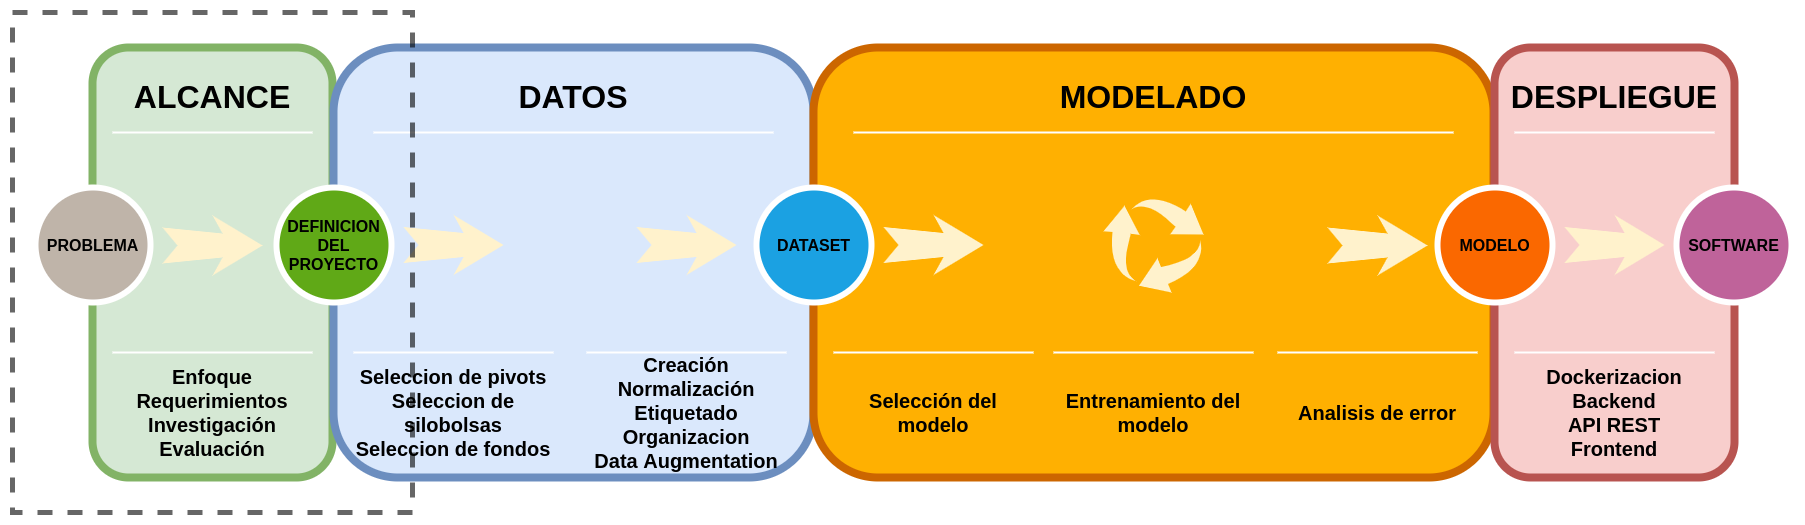
\includegraphics[width=1.2\textwidth,center]{img/Wokflow - alcance.drawio.png}
    \caption{Workflow: Alcance}
    \label{fig:workflow - alcance}
\end{figure}

\subsection{Entrevistas}

Las partes interesadas, como conocedores del área de las imágenes satelitales y del sector agropecuario, fueron entrevistadas con el objetivo de entender las primeras especificaciones para el prototipo planteado en la sección \ref{Implementación}. Para entender mejor los problemas del sistema de riego que se usa en el campo, como así también el almacenamiento de los cereales, legumbres, entre otros, y el uso de este prototipo junto con el beneficio del mismo para un futuro.

De la charla, se plantearon los siguientes problemas:
El primer problema es un problema de digitalización:
\begin{itemize}
    \begin{itemize}
        \item Deforestaciones ilegales
        \item Asentamientos ilegales y expropiaciones.
        \item Evasión impositivas en el rubro agropecuario.
        \item Abuso de los recursos hídricos.
    \end{itemize}
\end{itemize}

Las soluciones propuestas que surgieron de la entrevista fueron:
\begin{itemize}
    \item Debido a la fuerte influencia de algoritmos de Machine Learning de detección, se propuso hacer uso de esta tecnología para desarrollar una aplicación que provea lo siguiente:
    \begin{itemize}
        \item Detectar múltiples objetos, es este caso los objetos en cuestión son las silobolsas y los pivotes de riego.
        \item Dar la posición X e Y del objeto en la imagen (o su centro) y dibujar un rectángulo a su alrededor.
        \item Otra alternativa es Detectar “a tiempo”. Ésta es una característica que se debe tener en cuenta si por ejemplo se quiere hacer detección en tiempo real sobre vídeo.
        \item Otra de las propiedades de la detención de objetos que provee, es su carácter de velocidad y precisión para la detección. 
    \end{itemize}
\end{itemize}

\subsection{Motivación e Importancia del proyecto}

Ante las preocupaciones anteriormente planteadas, se propone una solución para satisfacer esas necesidades que no estaban cubiertas, por lo cual se enumeran a continuación las motivaciones que se presentaron para llevarlo a cabo:

\begin{enumerate}
    \item Elevar la inteligencia de la toma de acciones automáticas, por ejemplo, en un sistema de Dirección General de Rentas.
    \item Incorporar tecnologías novedosas y altamente populares en la industria al ámbito Agropecuario público.
    \item Ayudar a combatir irregularidades o deforestaciones detectándolas en tiempo real.
\end{enumerate}

\subsection{Casos de uso de Machine Learning - Detección de objetos}


Desde el éxito de Machine Learning y el nacimiento de numerosas aplicaciones que la usan, como el reconocimiento facial en tiempo real (celulares), sugerencias de compras, autos autónomos, entre otras, están, hoy en día, todas al alcance de cualquiera. Es una tecnología que está madura y es adoptada en la vida cotidiana.

Un claro ejemplo del alcance de la Inteligencia Artificial, es el motor de Google con aplicaciones de sistemas de inteligencia artificial y aprendizaje profundo, el cual ofrece respuestas adecuadas, tales como son las traducciones automáticas, las recomendaciones de vídeos, el reconocimiento de imágenes y su posterior geo-localización, y hasta la detección de SPAM (correo electrónico masivo no solicitado) en el correo electrónico.

Otro impacto de esta tecnología, es en el futuro de la conducción con Piloto automático en coches Tesla \cite{tesla}, por ejemplo, que vienen de serie con una combinación de hardware y software avanzado capaz de ofrecer las funciones de Piloto automático y capacidades de conducción autónoma total basado en una IA (Inteligencia Artificial) para la visión y la planificación.


\subsection{Funcionalidades}

Luego de la entrevista y de la evaluación del caso de uso, se consideran necesarias las siguientes funcionalidades para el prototipo:
\begin{itemize}
    \item El prototipo debe consistir de una API con una interfaz amigable para que cualquier usuario pueda procesar una imagen.
    \item El prototipo debe ser capaz que recibir imágenes de diferentes tamaños y características, ya sea por unidad o por cantidad en archivos comprimidos. A las que se le va aplicar el algoritmo de detección.
    \item El prototipo debe proporcionar como resultado del procesamiento, una imagen con con los objetos detectados remarcados con cuadros delimitadores y su localización en coordenadas (x,y). 
\end{itemize}

Este prototipo se realiza con una una API de REST, o API de RESTful \cite{api}, la cual es una interfaz de programación de aplicaciones (API o API web), que se ajusta a los límites de la arquitectura REST y permite la interacción con los servicios web de RESTful.

En otras palabras, las APIs le permiten interactuar con una computadora o un sistema para obtener datos o ejecutar una función, de manera que el sistema comprenda la solicitud y la cumpla. Suele considerarse como el contrato entre el proveedor de información y el usuario, donde se establece el contenido que se necesita por parte del consumidor (la llamada) y el que requiere el productor (la respuesta).

\\
\subsection{Definición de los Componentes}

Con el fin de implementar las funcionalidades descritas en la sección anterior, en primer lugar se definen los componentes del prototipo en su totalidad.

\begin{enumerate}

    \item \textbf{Elección del Modelo :} El modelo elegido luego de realizar varias pruebas y con el cual se obtuvieron los mejores resultados fue: YOLOv5, con un excelente rendimiento en la detección de objetos, en comparación a sus versiones anteriores.
    
    \item \textbf{Elección del lenguaje de programación:} El framework empleado para el entrenamiento y en el cual esta basado YOLOv5 \cite{yolov5} en Pytorch y Python.
    
    \item \textbf{Desarrollo de una API: }El código escrito en JavaScript es el código cliente que invoca al servidor. Para que sea accesible a través de Internet es necesario el desarrollo de una API REST, que permita llamar las funciones con métodos HTML. La herramienta elegida para esa tarea es Node.js, es un entorno en tiempo de ejecución multiplataforma para la capa del servidor basado en JavaScript. Node.js es a su vez un entorno controlado por eventos diseñado para crear aplicaciones escalables, permitiéndote establecer y gestionar múltiples conexiones al mismo tiempo y flexible para aplicaciones web y APIs.
    
    \item \textbf{Desarrollo de una GUI:} La API públicamente expuesta a Internet necesita un frontend, o una interfaz web, que acceda a ella. Su funcionalidad consiste en obtener información de la API y mostrarla de forma entendible para el usuario, como también obtener datos ingresados por el usuario y enviarlos para su procesamiento a la API.
    Para lograr eso, se decidió utilizar Bootstrap \cite{bootstrap}, donde las páginas que adaptan su contenido de forma dinámica a medida que reciben entradas del usuario, en vez de descargar páginas nuevas de un servidor. La herramienta proporciona plantillas para CSS y HTML que facilitan la colocación y el diseño de la página, las fuentes, los botones y los elementos de navegación, de modo que implementar con ella un diseño web moderno resulta muy sencillo.
    
    \item \textbf{Diagrama general de la arquitectura }
    \begin{figure}[h!]
        \centering
        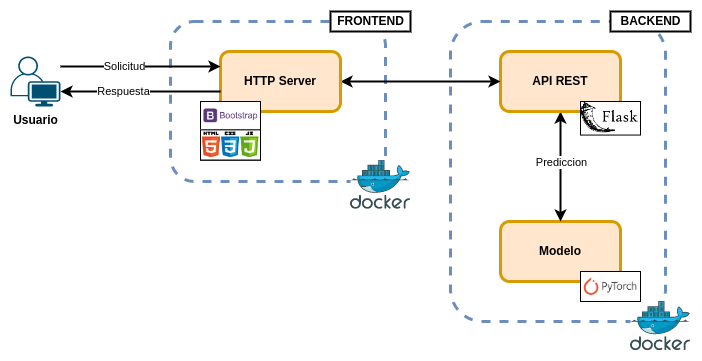
\includegraphics[width=1\textwidth,center]{img/BE - API - FE.drawio.png}
        \caption{Arquitectura del Software Implementado}
        \label{fig:be - api - fe}
    \end{figure}
    
    
\end{enumerate}

\newpage
\subsection{Definición de los Requerimientos}

Para especificar el funcionamiento general del sistema, se va a hacer uso del lenguaje de modelado UML. Si bien se trata del desarrollo de un sistema distribuido con una variedad de protocolos y tecnologı́as, el prototipo final es un producto de software, por lo cual un modelado en SysML \cite{sysml} no se consideró.

Antes de plantear los requerimientos, primero es necesario definir un diagrama de casos de uso, como se ve en la Figura \ref{fig:diagrama-casos-de-uso}. En el diagrama se puede observar que el objetivo principal es brindarle al usuario un sistema de detección de objetos sobre imágenes satelitales.


\subsubsection {Diagrama de casos de uso}

\begin{figure}[h!]
    \centering
    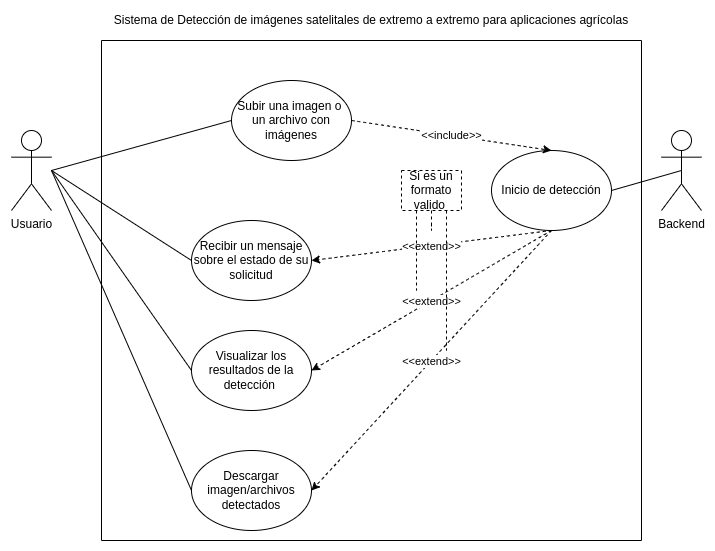
\includegraphics[width=1\textwidth]{img/Diagrama de Casos de usos.drawio (1).png}
    \caption{Diagrama de Caso de usos}
    \label{fig:diagrama-casos-de-uso}
\end{figure}

Con el diagrama de caso de uso elaborado se pueden definir los siguientes requerimientos de usuario, definidos en el Cuadro \ref{requser}:

\begin{table}[h!]
    \begin{tabular}{ | p{1cm} |p{11cm}| }
        \hline
        \rowcolor[HTML]{d6d8ff}
        R-01 & Cargar una imagen nueva al sistema.\\
        \hline
        R-02 & Verificar la presencia de una imagen cargada.\\
        \hline
        \rowcolor[HTML]{d6d8ff}
        R-03 & En caso de que sea un formato erróneo, mostrar un mensaje del error y debe ser posible volver a cargar una nueva imagen.\\
        \hline
        R-04 & Visualizar todas las imágenes cargadas y posteriormente un historial de las analizadas.\\
        \hline
        \rowcolor[HTML]{d6d8ff}
        R-05 & Analizar la imagen cargada, obtener información de la misma y el sistema debe informar si se encontró algún objeto o no.\\
        \hline
        R-06 & Descargar la imagen ya analizada.\\
        \hline
    \end{tabular}
    \caption{Requerimientos de Usuario}
    \label{requser}
\end{table}

\newpage
Luego es posible definir los requerimientos funcionales para cada uno de los componentes descritos anteriormente: la API y la interfaz gráfica. Los cuales se encuentran en los Cuadros \ref{reqapi} y \ref{reqfend} respectivamente. Los Requerimientos No funcionales se definieron en el Cuadro \ref{reqnf}.

\begin{table}[h!]
    \begin{tabular}{ | p{2cm} |p{10cm}| }
        \hline
        \rowcolor[HTML]{d6d8ff}
        RF-API-01 & Disponer de un endpoint para acceder a los servicios de detección.\\
        \hline
        RF-API-02 & Soportar una imagen y/o un archivo comprimido con imágenes.\\
        \hline
        \rowcolor[HTML]{d6d8ff}
         RF-API-03 & Realizar la detección de silobolsas y pivotes de riego sobre los archivos recibidos.\\
        \hline
         RF-API-04 & Retornar un archivos con la/s imágen/es con los objetos detectados.\\
        \hline
        \rowcolor[HTML]{d6d8ff}
         RF-API-05 & Retornar información adicional sobre la detección y el sistema donde fue ejecutado.\\
        \hline
    \end{tabular}\\
    \caption{Requerimientos Funcionales de la API}
    \label{reqapi}
\end{table}

\begin{table}[h!]
    \begin{tabular}{ | p{2cm} |p{10cm}| }
        \hline
        \rowcolor[HTML]{d6d8ff}
        RF-FE-01 & Mostrar información sobre el sistema y sus desarrolladores.\\
        \hline
        RF-FE-02 & Admitir carga de archivos.\\
        \hline
        \rowcolor[HTML]{d6d8ff}
        RF-FE-03 & Mostrar la imagen con los objetos detectados.\\
        \hline
        RF-FE-04 & Mostrar información de la detección.\\
        \hline
        \rowcolor[HTML]{d6d8ff}
        RF-FE-05 & Visualizar historial de la detecciones anteriores.\\
        \hline
        RF-FE-06 & Permitir la descarga de archivos.\\
        \hline
    \end{tabular}\\
    \caption{Requerimientos Funcionales del Frontend}
    \label{reqfend}
\end{table}

\begin{table}[h!]
    \begin{tabular}{ | p{2cm} |p{10cm}| }
        \hline
        \rowcolor[HTML]{d6d8ff}
        RNF-01 & Tiempo de detección menor a 100ms por imagen.\\
        \hline
        RNF-02 & Presentar una interfaz amigable para cualquier usuario.\\
        \hline
        \rowcolor[HTML]{d6d8ff}
        RNF-03 & Soportar diferentes formatos de archivos. \\
        \hline
        RNF-04 & Capacidad de ser desplegado fácilmente en diferentes sistemas\\
        \hline
        \rowcolor[HTML]{d6d8ff}
        RNF-05 & La API debe desarrollarse en Node.js y para la interfaz gráfica se debe usar CSS, HTML y JavaScript.\\
        \hline
    \end{tabular}\\
    \caption{Requerimientos No Funcionales del Sistema}
    \label{reqnf}
\end{table}

\newpage
Para comprender mejor cual es la relación estructural entre las diferentes tecnologı́as empleadas en el prototipo, se ofrece un diagrama de componentes, realizado en la Figura \ref{fig:componentes}. Se distinguen 3 componentes principales:
\begin{itemize}
    \item El Frontend donde se encuentra nuestra página web.
    \item La aplicación - API REST.
    \item El Modelo de Machine Learning - YOLOv5, donde los últimos dos componentes conforman el Backend.
\end{itemize}

\begin{figure}[h!]
    \centering
    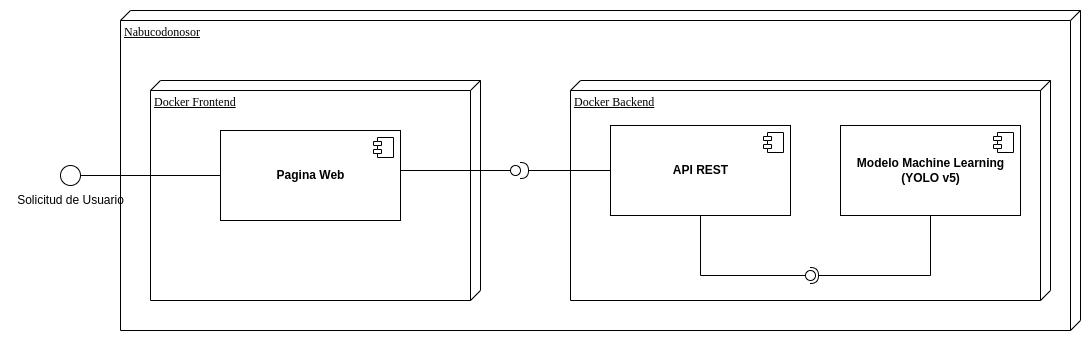
\includegraphics[width=1\textwidth]{img/Diagrama de Componentes.drawio.png}
    \caption{Diagrama de Componentes}
    \label{fig:componentes}
\end{figure}

\newpage
\subsection{Definición del Comportamiento}

Para entender cómo interactúan los componentes diagramados, se emplea un diagrama de secuencia en la Figura \ref{fig:secuencia}, en el cual se muestra el flujo de mensajes para el caso de subir una imagen a analizar y su posterior descarga, como también para verificar la validez del formato de una imagen y en caso de ser válido, proveer los resultados de las detecciones correspondientes.

\begin{figure}[h!]
    \centering
    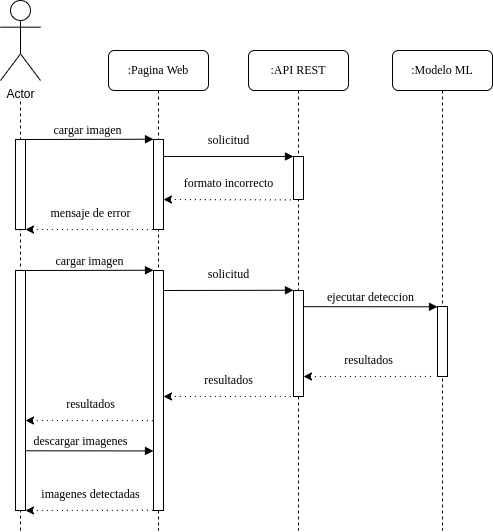
\includegraphics[width=0.9\textwidth]{img/Diagrama de Secuencia.drawio.png}
    \caption{Diagrama de Secuencia}
    \label{fig:secuencia}
\end{figure}


\subsection{Riesgos}

La evaluación de riesgos de un proyecto busca detectar posibles eventos no deseados que puedan perjudicar o amenazar al proyecto, con el objetivo de minimizarlos o controlar su impacto sobre el proyecto.

En la presente sección se establecen diferentes criterios para identificar posibles riesgos, asignar prioridades a los mismos, evaluar su probabilidad y encontrar estrategias que permitan resolver los mismos o minimizar sus efectos.


\subsubsection{Criterios}

Los riesgos se clasifican según dos criterios: su probabilidad y la gravedad en el caso de su ocurrencia. A continuación, figuran las probabilidades y gravedades que se tuvieron en cuenta según Ian Sommerville en su libro Software Engineering \cite{sommerville}:

\begin{enumerate}
    \item Riesgo muy bajo (menor a 10 \%)
    \item Riesgo bajo (10 - 25 \%)
    \item Riesgo moderado (25 - 50 \%)
    \item Riesgo alto (50 - 75 \%)
    \item Riesgo muy alto (mayor a 75 \%)
\end{enumerate}

\begin{enumerate}
    \item Efectos insignificantes
    \item Efectos tolerables
    \item Efectos graves
    \item Efectos catastróficos
\end{enumerate}

La combinación de ambos criterios permite detectar y priorizar los riesgos teniendo en cuenta ambos factores, y se consideran a los riesgos dentro del área verde como los de menor prioridad, los riesgos en el área amarilla como de prioridad intermedia y los riesgos en el área roja como de prioridad alta, como se muestra en el Cuadro \ref{probriesgos}.

\begin{table}[h]
    \begin{tabular}{ | m{3cm} | m{3cm}| m{2cm} | m{2cm} |m{2cm} |}
        \hline
        Probabilidad-Efecto & Insignificante & Tolerable &Grave & Catastrófico\\
        \hline
        Muy baja& \cellcolor[HTML]{84D65C} & \cellcolor[HTML]{84D65C}&\cellcolor[HTML]{84D65C} &\cellcolor[HTML]{FFFF00}\\
        \hline
        Baja & \cellcolor[HTML]{84D65C} & \cellcolor[HTML]{84D65C}&\cellcolor[HTML]{FFFF00} &\cellcolor[HTML]{FFFF00}\\
        \hline
        Moderada& \cellcolor[HTML]{84D65C} &\cellcolor[HTML]{FFFF00} &\cellcolor[HTML]{FFFF00} &\cellcolor[HTML]{FF3333} \\
        \hline
        Alta  &\cellcolor[HTML]{FFFF00}  &\cellcolor[HTML]{FFFF00} & \cellcolor[HTML]{FF3333} &\cellcolor[HTML]{FF3333} \\
        \hline
        Muy alta & \cellcolor[HTML]{FFFF00} &\cellcolor[HTML]{FF3333}  & \cellcolor[HTML]{FF3333} &\cellcolor[HTML]{FF3333} \\
        \hline
    \end{tabular}\\
    \caption{Probabilidad de Riesgos Vs Efecto}
    \label{probriesgos}
\end{table}

\subsubsection{Identificación de Riesgos}

En la etapa de la gestión de riesgos, se buscan los posibles riesgos relacionados al proyecto escritos en el Cuadro \ref{riesgosproyecto}, distinguiendo las siguientes categorías :
\begin{itemize}
    \item \textbf{Riesgos de tecnologı́a}: Riesgos relacionados la hardware o software con el que se está desarrollando el presente proyecto.
    \item \textbf{Riesgos personales:} Relacionados con lo personal del equipo de desarrollo.
    \item \textbf{Riesgos de requerimientos:} Surgen de modificaciones de los requerimientos.
    \item \textbf{Riesgos de estimación:} relacionados a la estimación de recursos requeridos o estimación de tiempo para el desarrollo del proyecto.
\end{itemize}

\begin{table}[h]
    \begin{tabular}{ | m{1.5cm} | m{7cm}| m{3.5cm}  |}
        \hline
        \rowcolor{lightgray}
        Código & Descripción & Tipo de Riesgo \\
        \hline
        Riesgo-01 & Problemas de funcionamiento o fuera de servicio de la Máquina donde se desarrolla el proyecto  & Tecnológico \\
        \hline
        Riesgo-02 & Incompatibilidad de versiones o librerı́as instaladas en la máquina de desarrollo con los frameworks usados.  &Tecnológico \\
        \hline
        Riesgo-03 & Demoras durante el desarrollo del proyecto debido a trabajo u otros inconvenientes personales.  &  Personales y Estimación\\
        \hline
        Riesgo-04 & Errores en la implementación de los frameworks elegidos.  & Tecnológico, Requerimientos y Estimación\\
        \hline
        Riesgo-05 & Falta de conocimiento o documentación para el uso de los frameworks, del software o los lenguajes de programación elegidos.  & Estimación\\
        \hline
        Riesgo-06 & Rechazo de la implementación por parte del usuario final.  & Estimación\\
        \hline
    \end{tabular}\\
    \caption{Riesgos identificados para el proyecto}
    \label{riesgosproyecto}
\end{table}

\newpage
\subsubsection{Análisis de Riesgos}

En el Cuadro \ref{riesgosprobyefecto} se ordenaron los riesgos según su importancia, probabilidad y efecto.

\begin{table}[h!]
    \begin{tabular}{ | m{1.5cm} | m{4cm}|m{2cm}  | m{2cm}  | m{2cm}  |}
        \hline
        \rowcolor{lightgray}
        Código & Riesgo & Probabilidad & Efecto & Importancia \\
        \hline
        Riesgo-02 & Incompatibilidad de versiones o librerı́as instaladas en la máquina de desarrollo con los frameworks usados. & Moderada &Insignificante&
        \cellcolor[HTML]{84D65C} Prioridad baja \\
        \hline
        Riesgo-01 & Problemas de funcionamiento o fuera de servicio de la Máquina donde se desarrolla el proyecto & Baja &Grave & \cellcolor[HTML]{FFFF00} Prioridad Intermedia\\
        \hline
        Riesgo-05 & Falta de conocimiento o documentación para el uso de los frameworks, del software o los lenguajes de programación elegidos.
         & Alta   & Tolerable& \cellcolor[HTML]{FFFF00} Prioridad Intermedia\\
        \hline
        Riesgo-04  & Errores en la implementación de los frameworks elegidos.  & Alta  &Tolerable &\cellcolor[HTML]{FFFF00} Prioridad intermedia\\
        \hline
         Riesgo-03 & Demoras durante el desarrollo del proyecto debido a trabajo u otros inconvenientes personales.  & Alta  &Grave & \cellcolor[HTML]{FF3333} Prioridad alta\\
        \hline
        Riesgo-06 & Rechazo de la implementación por parte del usuario final.  & Alta  &Grave & \cellcolor[HTML]{FF3333} Prioridad alta\\
        \hline
    \end{tabular}\\
    \caption{Riesgos según su probabilidad y efecto}
    \label{riesgosprobyefecto}
\end{table}

\newpage
\subsubsection{Planificación de Riesgos}

En la presente sección se describen las estrategias para manejar cada riesgo identificado anteriormente, y se detallan en los Cuadros \ref{manejoriesgos1} y \ref{manejoriesgos2}.

\begin{table}[h!]
    \begin{tabular}{ | m{1.5cm} | m{5cm}| m{5cm} |}
        \hline
        \textbf{Código} & \textbf{Riesgo} & \textbf{Probabilidad} \\
        \hline
        Riesgo-01 & Problemas de funcionamiento o fuera de servicio de la Máquina donde se desarrolla el proyecto  & \begin{itemize}
         \item Implementación de un respaldo de información en la nube con repositorios de Github.
            \item Realización de la operación \textit{git push} al repositorio diariamente o ante algún cambio. 
             \end{itemize}\\
        \hline
         Riesgo-02 & Incompatibilidad de versiones o librerı́as instaladas en la máquina de desarrollo con los frameworks usados.&  \begin{itemize}
         \item Lectura cuidadosa de tutoriales de instalación y pre-requisitos.     
         \item Uso de Docker para ganar mayor flexibilidad con versiones de librerı́as o lenguajes de programación. 
         \end{itemize} \\
        \hline
         Riesgo-03 & Demoras durante el desarrollo del proyecto debido a trabajo u otros inconvenientes personales.    
         & \begin{itemize} 
            \item Comunicación fluida con director y codirector del Proyecto.    
            \item Reducción de obligaciones laborales y extracurriculares. 
            \item Definición clara del alcance del proyecto para minimizar las posibles demoras de tiempo y trabajo.
          \end{itemize}\\
        \hline
        Riesgo-04 & Errores en la implementación de los frameworks elegidos.  &
        \begin{itemize} 
                    \item Implementación de métodos descritos en la documentación o páginas de seguimientos, como también foros oficiales.
                    \item Modificación o adaptación del requerimiento y su implementación.
                \end{itemize}\\
        \hline
    \end{tabular}\\
    \caption{Estrategias de manejo de riesgos - Parte 1}
    \label{manejoriesgos1}
\end{table}


\begin{table}[h!]
    \begin{tabular}{ | m{1.5cm} | m{5cm}| m{5cm} |}
        \hline
        \textbf{Código} & \textbf{Riesgo} & \textbf{Probabilidad} \\
        \hline
         Riesgo-05 & Falta de conocimiento o documentación para el uso de los frameworks, del software o los lenguajes de programación elegidos.&  \begin{itemize} 
                    \item Lectura de tutoriales y realización de cursos cortos para lograr una introducción en temas cuyo desconocimiento impida el avance del proyecto.
                    \item Empleo y modificación/adaptación de ejemplos previstos para el aprendizaje.
                    \item Búsqueda de explicaciones adicionales en foros de usuarios como StackOverflow \cite{stackoverflow}.
                    \item Consultas a programadores o profesionales experimentados en los campos en cuestión.
                \end{itemize}\\
        \hline
        Riesgo-06 &Rechazo de la implementación por parte del usuario final.  & 
        \begin{itemize} 
            \item Explicación de la tecnologı́a empleada y proporcionar manual de usuario para su uso.
            \item  Prueba de piloto para identificar mejoras en cuanto a la usabilidad y posibilidad de mejoras en un futuro.
                \end{itemize}\\
        \hline
    \end{tabular}\\
    \caption{Estrategias de manejo de riesgos - Parte 2}
    \label{manejoriesgos2}
\end{table}

\newpage
\subsection{Control de Versiones }
Git es una herramienta para mejorar la colaboración entre varios programadores. Usar un repositorio permite tener acceso remoto al proyecto desde cualquier equipo, teniendo ası́ una copia de seguridad del proyecto completo en la nube. A su vez, se mantiene un historial de versiones y en caso de ser necesario, volver a una versión anterior o comparar las diferencias entre dos versiones distintas.

Para el control de versiones, se utilizó un repositorio de Github disponible bajo la URL:  \url{https://github.com/gianfrancob/detector_pivotes_silobolsas}
\newpage
